% Options for packages loaded elsewhere
% Options for packages loaded elsewhere
\PassOptionsToPackage{unicode}{hyperref}
\PassOptionsToPackage{hyphens}{url}
\PassOptionsToPackage{dvipsnames,svgnames,x11names}{xcolor}
%
\documentclass[
  12pt,
  letterpaper,
]{article}
\usepackage{xcolor}
\usepackage[margin=1in]{geometry}
\usepackage{amsmath,amssymb}
\setcounter{secnumdepth}{-\maxdimen} % remove section numbering
\usepackage{iftex}
\ifPDFTeX
  \usepackage[T1]{fontenc}
  \usepackage[utf8]{inputenc}
  \usepackage{textcomp} % provide euro and other symbols
\else % if luatex or xetex
  \usepackage{unicode-math} % this also loads fontspec
  \defaultfontfeatures{Scale=MatchLowercase}
  \defaultfontfeatures[\rmfamily]{Ligatures=TeX,Scale=1}
\fi
\usepackage{lmodern}
\ifPDFTeX\else
  % xetex/luatex font selection
\fi
% Use upquote if available, for straight quotes in verbatim environments
\IfFileExists{upquote.sty}{\usepackage{upquote}}{}
\IfFileExists{microtype.sty}{% use microtype if available
  \usepackage[]{microtype}
  \UseMicrotypeSet[protrusion]{basicmath} % disable protrusion for tt fonts
}{}
\makeatletter
\@ifundefined{KOMAClassName}{% if non-KOMA class
  \IfFileExists{parskip.sty}{%
    \usepackage{parskip}
  }{% else
    \setlength{\parindent}{0pt}
    \setlength{\parskip}{6pt plus 2pt minus 1pt}}
}{% if KOMA class
  \KOMAoptions{parskip=half}}
\makeatother
% Make \paragraph and \subparagraph free-standing
\makeatletter
\ifx\paragraph\undefined\else
  \let\oldparagraph\paragraph
  \renewcommand{\paragraph}{
    \@ifstar
      \xxxParagraphStar
      \xxxParagraphNoStar
  }
  \newcommand{\xxxParagraphStar}[1]{\oldparagraph*{#1}\mbox{}}
  \newcommand{\xxxParagraphNoStar}[1]{\oldparagraph{#1}\mbox{}}
\fi
\ifx\subparagraph\undefined\else
  \let\oldsubparagraph\subparagraph
  \renewcommand{\subparagraph}{
    \@ifstar
      \xxxSubParagraphStar
      \xxxSubParagraphNoStar
  }
  \newcommand{\xxxSubParagraphStar}[1]{\oldsubparagraph*{#1}\mbox{}}
  \newcommand{\xxxSubParagraphNoStar}[1]{\oldsubparagraph{#1}\mbox{}}
\fi
\makeatother


\usepackage{longtable,booktabs,array}
\newcounter{none} % for unnumbered tables
\usepackage{calc} % for calculating minipage widths
% Correct order of tables after \paragraph or \subparagraph
\usepackage{etoolbox}
\makeatletter
\patchcmd\longtable{\par}{\if@noskipsec\mbox{}\fi\par}{}{}
\makeatother
% Allow footnotes in longtable head/foot
\IfFileExists{footnotehyper.sty}{\usepackage{footnotehyper}}{\usepackage{footnote}}
\makesavenoteenv{longtable}
\usepackage{graphicx}
\makeatletter
\newsavebox\pandoc@box
\newcommand*\pandocbounded[1]{% scales image to fit in text height/width
  \sbox\pandoc@box{#1}%
  \Gscale@div\@tempa{\textheight}{\dimexpr\ht\pandoc@box+\dp\pandoc@box\relax}%
  \Gscale@div\@tempb{\linewidth}{\wd\pandoc@box}%
  \ifdim\@tempb\p@<\@tempa\p@\let\@tempa\@tempb\fi% select the smaller of both
  \ifdim\@tempa\p@<\p@\scalebox{\@tempa}{\usebox\pandoc@box}%
  \else\usebox{\pandoc@box}%
  \fi%
}
% Set default figure placement to htbp
\def\fps@figure{htbp}
\makeatother


% definitions for citeproc citations
\NewDocumentCommand\citeproctext{}{}
\NewDocumentCommand\citeproc{mm}{%
  \begingroup\def\citeproctext{#2}\cite{#1}\endgroup}
\makeatletter
 % allow citations to break across lines
 \let\@cite@ofmt\@firstofone
 % avoid brackets around text for \cite:
 \def\@biblabel#1{}
 \def\@cite#1#2{{#1\if@tempswa , #2\fi}}
\makeatother
\newlength{\cslhangindent}
\setlength{\cslhangindent}{1.5em}
\newlength{\csllabelwidth}
\setlength{\csllabelwidth}{3em}
\newenvironment{CSLReferences}[2] % #1 hanging-indent, #2 entry-spacing
 {\begin{list}{}{%
  \setlength{\itemindent}{0pt}
  \setlength{\leftmargin}{0pt}
  \setlength{\parsep}{0pt}
  % turn on hanging indent if param 1 is 1
  \ifodd #1
   \setlength{\leftmargin}{\cslhangindent}
   \setlength{\itemindent}{-1\cslhangindent}
  \fi
  % set entry spacing
  \setlength{\itemsep}{#2\baselineskip}}}
 {\end{list}}
\usepackage{calc}
\newcommand{\CSLBlock}[1]{\hfill\break\parbox[t]{\linewidth}{\strut\ignorespaces#1\strut}}
\newcommand{\CSLLeftMargin}[1]{\parbox[t]{\csllabelwidth}{\strut#1\strut}}
\newcommand{\CSLRightInline}[1]{\parbox[t]{\linewidth - \csllabelwidth}{\strut#1\strut}}
\newcommand{\CSLIndent}[1]{\hspace{\cslhangindent}#1}



\setlength{\emergencystretch}{3em} % prevent overfull lines

\providecommand{\tightlist}{%
  \setlength{\itemsep}{0pt}\setlength{\parskip}{0pt}}



 


\usepackage[bottom]{footmisc}
\usepackage{setspace}
\usepackage{parskip}
\setlength{\parindent}{20pt}
\usepackage{sectsty}
\sectionfont{\fontsize{12}{15}\selectfont}
\subsectionfont{\fontsize{12}{15}\selectfont}
\usepackage{fancyhdr}
\fancyhead{}
\fancyhead[L]{\small\textit{Work in progress. Please do not circulate.}}
\pagestyle{fancy}
\renewcommand{\headrulewidth}{0pt}
\makeatletter
\@ifpackageloaded{caption}{}{\usepackage{caption}}
\AtBeginDocument{%
\ifdefined\contentsname
  \renewcommand*\contentsname{Table of contents}
\else
  \newcommand\contentsname{Table of contents}
\fi
\ifdefined\listfigurename
  \renewcommand*\listfigurename{List of Figures}
\else
  \newcommand\listfigurename{List of Figures}
\fi
\ifdefined\listtablename
  \renewcommand*\listtablename{List of Tables}
\else
  \newcommand\listtablename{List of Tables}
\fi
\ifdefined\figurename
  \renewcommand*\figurename{Fig.}
\else
  \newcommand\figurename{Fig.}
\fi
\ifdefined\tablename
  \renewcommand*\tablename{Table}
\else
  \newcommand\tablename{Table}
\fi
}
\@ifpackageloaded{float}{}{\usepackage{float}}
\floatstyle{ruled}
\@ifundefined{c@chapter}{\newfloat{codelisting}{h}{lop}}{\newfloat{codelisting}{h}{lop}[chapter]}
\floatname{codelisting}{Listing}
\newcommand*\listoflistings{\listof{codelisting}{List of Listings}}
\makeatother
\makeatletter
\makeatother
\makeatletter
\@ifpackageloaded{caption}{}{\usepackage{caption}}
\@ifpackageloaded{subcaption}{}{\usepackage{subcaption}}
\makeatother
\usepackage{bookmark}
\IfFileExists{xurl.sty}{\usepackage{xurl}}{} % add URL line breaks if available
\urlstyle{same}
\hypersetup{
  pdftitle={Greening while Governing the Economy: Central Banks Matter to Decarbonization},
  pdfauthor={Vitor M. Dias},
  colorlinks=true,
  linkcolor={blue},
  filecolor={Maroon},
  citecolor={Blue},
  urlcolor={blue},
  pdfcreator={LaTeX via pandoc}}


\title{Greening while Governing the Economy:\\
Central Banks Matter to Decarbonization\thanks{Acknowledgements.}}
\author{Vitor M. Dias}
\date{}
\begin{document}
\maketitle
\begin{abstract}
Why do some countries translate international climate commitments into
emissions reductions while others do not? I test whether the answer lies
in central bank regulatory and governance powers. Membership in the
Network for Greening the Financial System (NGFS)---a voluntary
international network---is used as a measure of climate-oriented
financial governance across 145 countries from 2013 to 2023. Two-way
fixed-effects models and doubly robust difference-in-differences
estimates show that NGFS membership reduces within-country emissions by
4 to 9 percent, depending on the modeling technique employed. The effect
is small where central banks have low independence from political
authority and nearly doubles where independence is high. Mediation
analysis is consistent with independence functioning as a precondition
for the network's effectiveness rather than a consequence of membership.
International regulatory networks matter for decarbonization, but only
where domestic institutions, statutes, and regulations allow central
banks to act.
\end{abstract}


\newpage{}

Why do some countries translate international climate commitments into
emissions reductions while others do not? One answer relates to the role
central banks play in directing investments to low-carbon markets
(\emph{1}--\emph{4}). Central banks regulate how trillions of dollars
flow from banks and investment funds into the economy, governing which
sectors receive capital and according to what rules, statutes, and norms
(\emph{5}--\emph{8}). Yet, whether and how financial supervisors
facilitate or hinder the low-carbon transition remains an ongoing
discussion (\emph{1}--\emph{4}, \emph{9}, \emph{10}). I illuminate this
discussion by estimating the extent to which nations internationally
committed to ``green'' their central banks emit less greenhouse gases
(GHG) than nations with conventional central banks.

Addressing the question above by focusing on financial supervisors has
pressing policy implications. Confronting the climate crisis requires
decarbonizing not only factories, value chains, and power grids but also
the financial systems that fund them. A challenge for the empirical
analysis of central banks' influence on decarbonizing the global economy
is that no consistent cross-national marker has distinguished countries
with ``green'' central banks from nations with conventional ones. This
changed in 2017, when the Network of Central Banks and Supervisors for
Greening the Financial System (NGFS) was established (\emph{10},
\emph{11}).

The NGFS offers the first public registry of financial regulators
formally and internationally committed to integrating climate risks into
macroeconomic supervision (\emph{11}). Using NGFS membership as a
treatment indicator, I compare GHG emission trajectories across 145
countries from 2013 to 2023 (\(N = 1,595\)). To account for the fact
that countries joined the NGFS in different years---i.e., staggered
treatment timing---,I employ the Callaway and Sant'Anna (\emph{12})
doubly robust estimator, which isolates cohort-specific treatment
effects and is robust to the heterogeneous treatment timing that
standard two-way fixed effects models fail to handle without bias.
Difference-in-differences models with two-way fixed effects reveal that,
within countries, joining the NGFS is associated with a subsequent
deceleration in emission growth. This reduction ranges from
approximately 4\% to 9\% lower emissions relative to what within-country
trends would otherwise predict, after controlling for economic,
ecological, and political factors.

The effect above grows with central bank independence (\emph{13},
\emph{14}). NGFS membership carries little measurable impact where
central banks lack insulation from executive control, but becomes
substantial where bureaucratic autonomy (\emph{15}) to act independently
from executive overreach is high (\emph{16}). Institutional capacity to
implement policies (\emph{17}) aimed at managing environmental
externalities independently from partisan pressures helps reduce
emissions. Central bank independence and its limits are often defined by
statutes (\emph{18}). This process entails deliberations between members
of the executive and legislative powers (\emph{19}), which can
ultimately end in court (\emph{20}), making it challenging for political
leaders to undermine such regulatory powers (\emph{16}).\footnote{But
  see Fernandéz-Albertos (\emph{19}) for a discussion of the potential
  politicization of central banks.} These findings suggest that
participation in international regulatory networks, conditioned by
domestic institutional capacity and bureaucratic autonomy, shapes how
financial regulation can contribute to decarbonization.

\subsection{Central Banks, Climate Change, and Economic
Policy}\label{central-banks-climate-change-and-economic-policy}

Central banks and financial supervisors shape where capital goes. By
issuing prudential rules and regulations with which banks and investment
funds must comply, central banks govern which sectors of the real
economy receive financing (\emph{8}). This feature has been historically
documented when nations prioritized industrial, carbon-intensive
development (\emph{5}, \emph{7}, \emph{21}). As climate risks have
emerged as a recognized systemic financial risk (\emph{1}, \emph{22}),
central banks have increasingly been called upon to extend its
regulatory powers toward decarbonization (\emph{3}, \emph{4},
\emph{23}). The NGFS---established at the Paris ``One Planet Summit'' in
2017 and spearheaded by financial supervisors from France, China,
England, Germany, Mexico, Norway, Singapore, and Sweden---has worked to
build a coordinating infrastructure for climate-aligned financial
supervision (\emph{10}, \emph{11}).

Financial regulators that join the NGFS commit to integrating climate
scenarios into financial supervision and to standardizing the
classification of ``green'' and ``brown'' assets (\emph{1}, \emph{11}).
One goal is to facilitate capital reallocation from carbon-intensive
(i.e., ``brown'') to low-carbon (i.e., ``green'') ventures. Some NGFS
members have translated these commitments into binding domestic
regulations. For example, in 2021, Brazil's central bank mandated that
financial institutions disclose climate liabilities under their Social,
Environmental, and Climate Responsibility Policy (PRSAC)\footnote{In
  Portuguese, PRSAC refers to Política de Responsabilidade Social,
  Ambiental e Climática.} documents (\emph{16}). The Brazilian central
bank relied on its bureaucratic autonomy to implement policies without
executive interference (\emph{16}). By contrast, the U.S. Federal
Reserve---constrained by political opposition---joined the NGFS only
during the Biden administration (\emph{16}). This contrast illustrates
that central bank independence (\emph{14}) is not merely a macroeconomic
property but a precondition for effective climate governance.

A natural skeptical reaction to such international commitments is that
NGFS membership might represent ``performative governance'' (\emph{24},
\emph{25}). That is, in response to their citizens' pressure, wealthy,
industrialized nations that have already been on a decarbonization path
may have joined the NGFS because the costs of membership were low and
the reputational benefits were high. Based on this argument, any
observed emissions gap between NGFS members and non-members would
reflect pre-existing trajectories rather than an effect stemming from
NGFS participation. This concern is compounded by the network's initial
geographic concentration in the Global North (see
Fig.~\ref{fig-comb-plot}), where decarbonization pressures from domestic
constituencies, regional regulators, and capital markets were already
substantial before 2017. Importantly, as panel B of
Fig.~\ref{fig-comb-plot} shows, observed emission trajectories show that
NGFS members were, in fact, larger emitters than non-members before
2017, with a modest, almost imperceptible downward trend among nations
that joined the NGFS in 2017-2018. If wealthy, already-greening nations
had self-selected into the network, a steeper downward trajectory would
be expected instead.

\begin{figure}[H]

\centering{

\pandocbounded{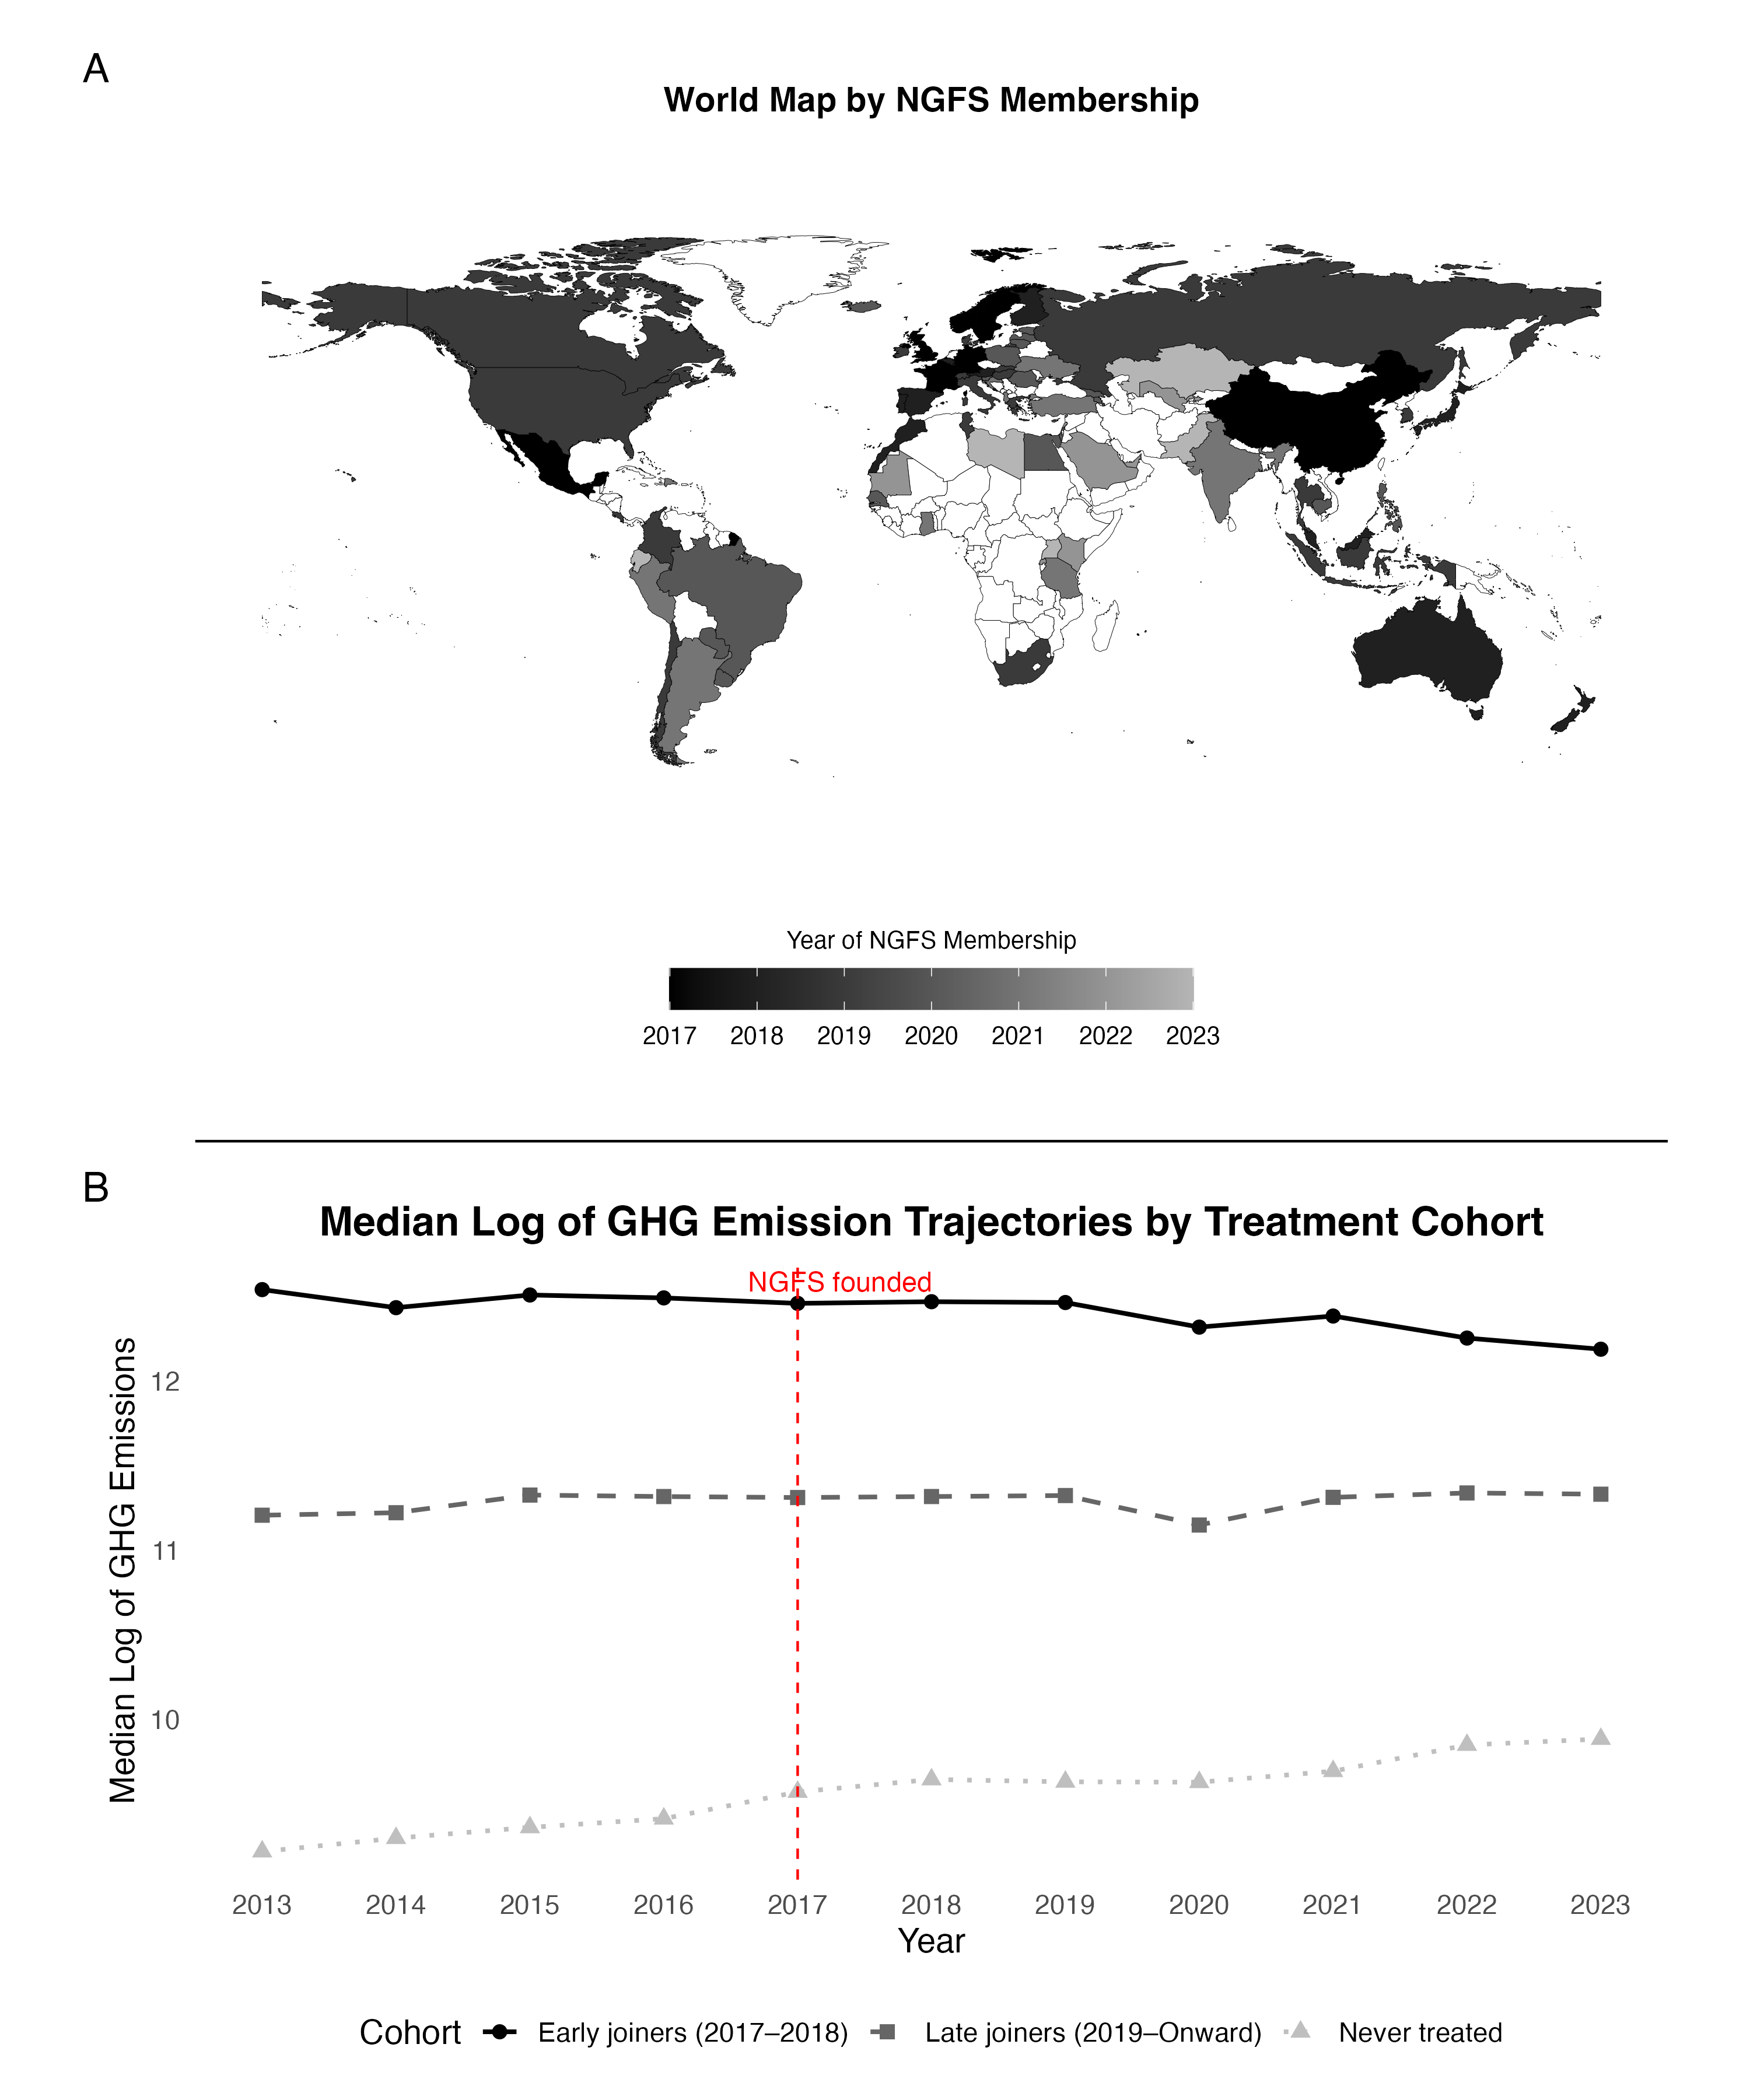
\includegraphics[keepaspectratio]{comb_map_cohort.png}}

}

\caption{\label{fig-comb-plot}}

\end{figure}%

A rigorous empirical test must nonetheless account for systematic
differences between early joiners (2017-2018), late joiners
(2018-onward), and never-treated countries. This step would address
selection bias concerns and help demonstrate that any post-membership
emissions deceleration exceeds what pre-existing within-country trends
would predict. I conduct such analysis using panel data from 145
countries between 2013 and 2023. As I demonstrate, NGFS membership is
associated with lower within-country emissions. Additionally, central
bank independence moderates the magnitude of the emissions effect that
NGFS membership can realistically produce.

\subsection{Results}\label{sec-results}

\textbf{\emph{NGFS membership is associated with lower within-country
emissions across multiple specifications}}

To estimate the effect of joining the NGFS on national GHG emissions, I
fit a series of two-way fixed effects (TWFE) models with country and
year fixed effects. Country-level fixed effects absorb time-invariant
differences across nations, e.g., natural resources characteristics and
institutional developmental paths. Year-level fixed effects account for
global shocks common to all countries simultaneously, including economic
downturns, global pandemics, and multilateral climate agreements, such
as the Paris Agreement. Accordingly, the identifying variation in the
models is within-country: changes in emissions trajectories following
NGFS entry, relative to never-treated countries in the same years.

I assess the effect across three outcomes: total GHG emissions,
emissions normalized by GDP per capita, and emissions per capita. All
models control for economic, ecological, and political variables, such
as trade openness, land use, and institutional capacity.
Fig.~\ref{fig-feplot} shows that NGFS membership is associated with a
statistically significant within-country reduction in emissions across
all three specifications. Point estimates range from approximately 4\%
to 9\% lower emissions among NGFS members compared to non-members, all
else equal. Despite differences in the confidence intervals when
emissions are normalized by population or GDP per capita, the direction
and significance of the effect are consistent across specifications.

\begin{figure}[H]

\centering{

\pandocbounded{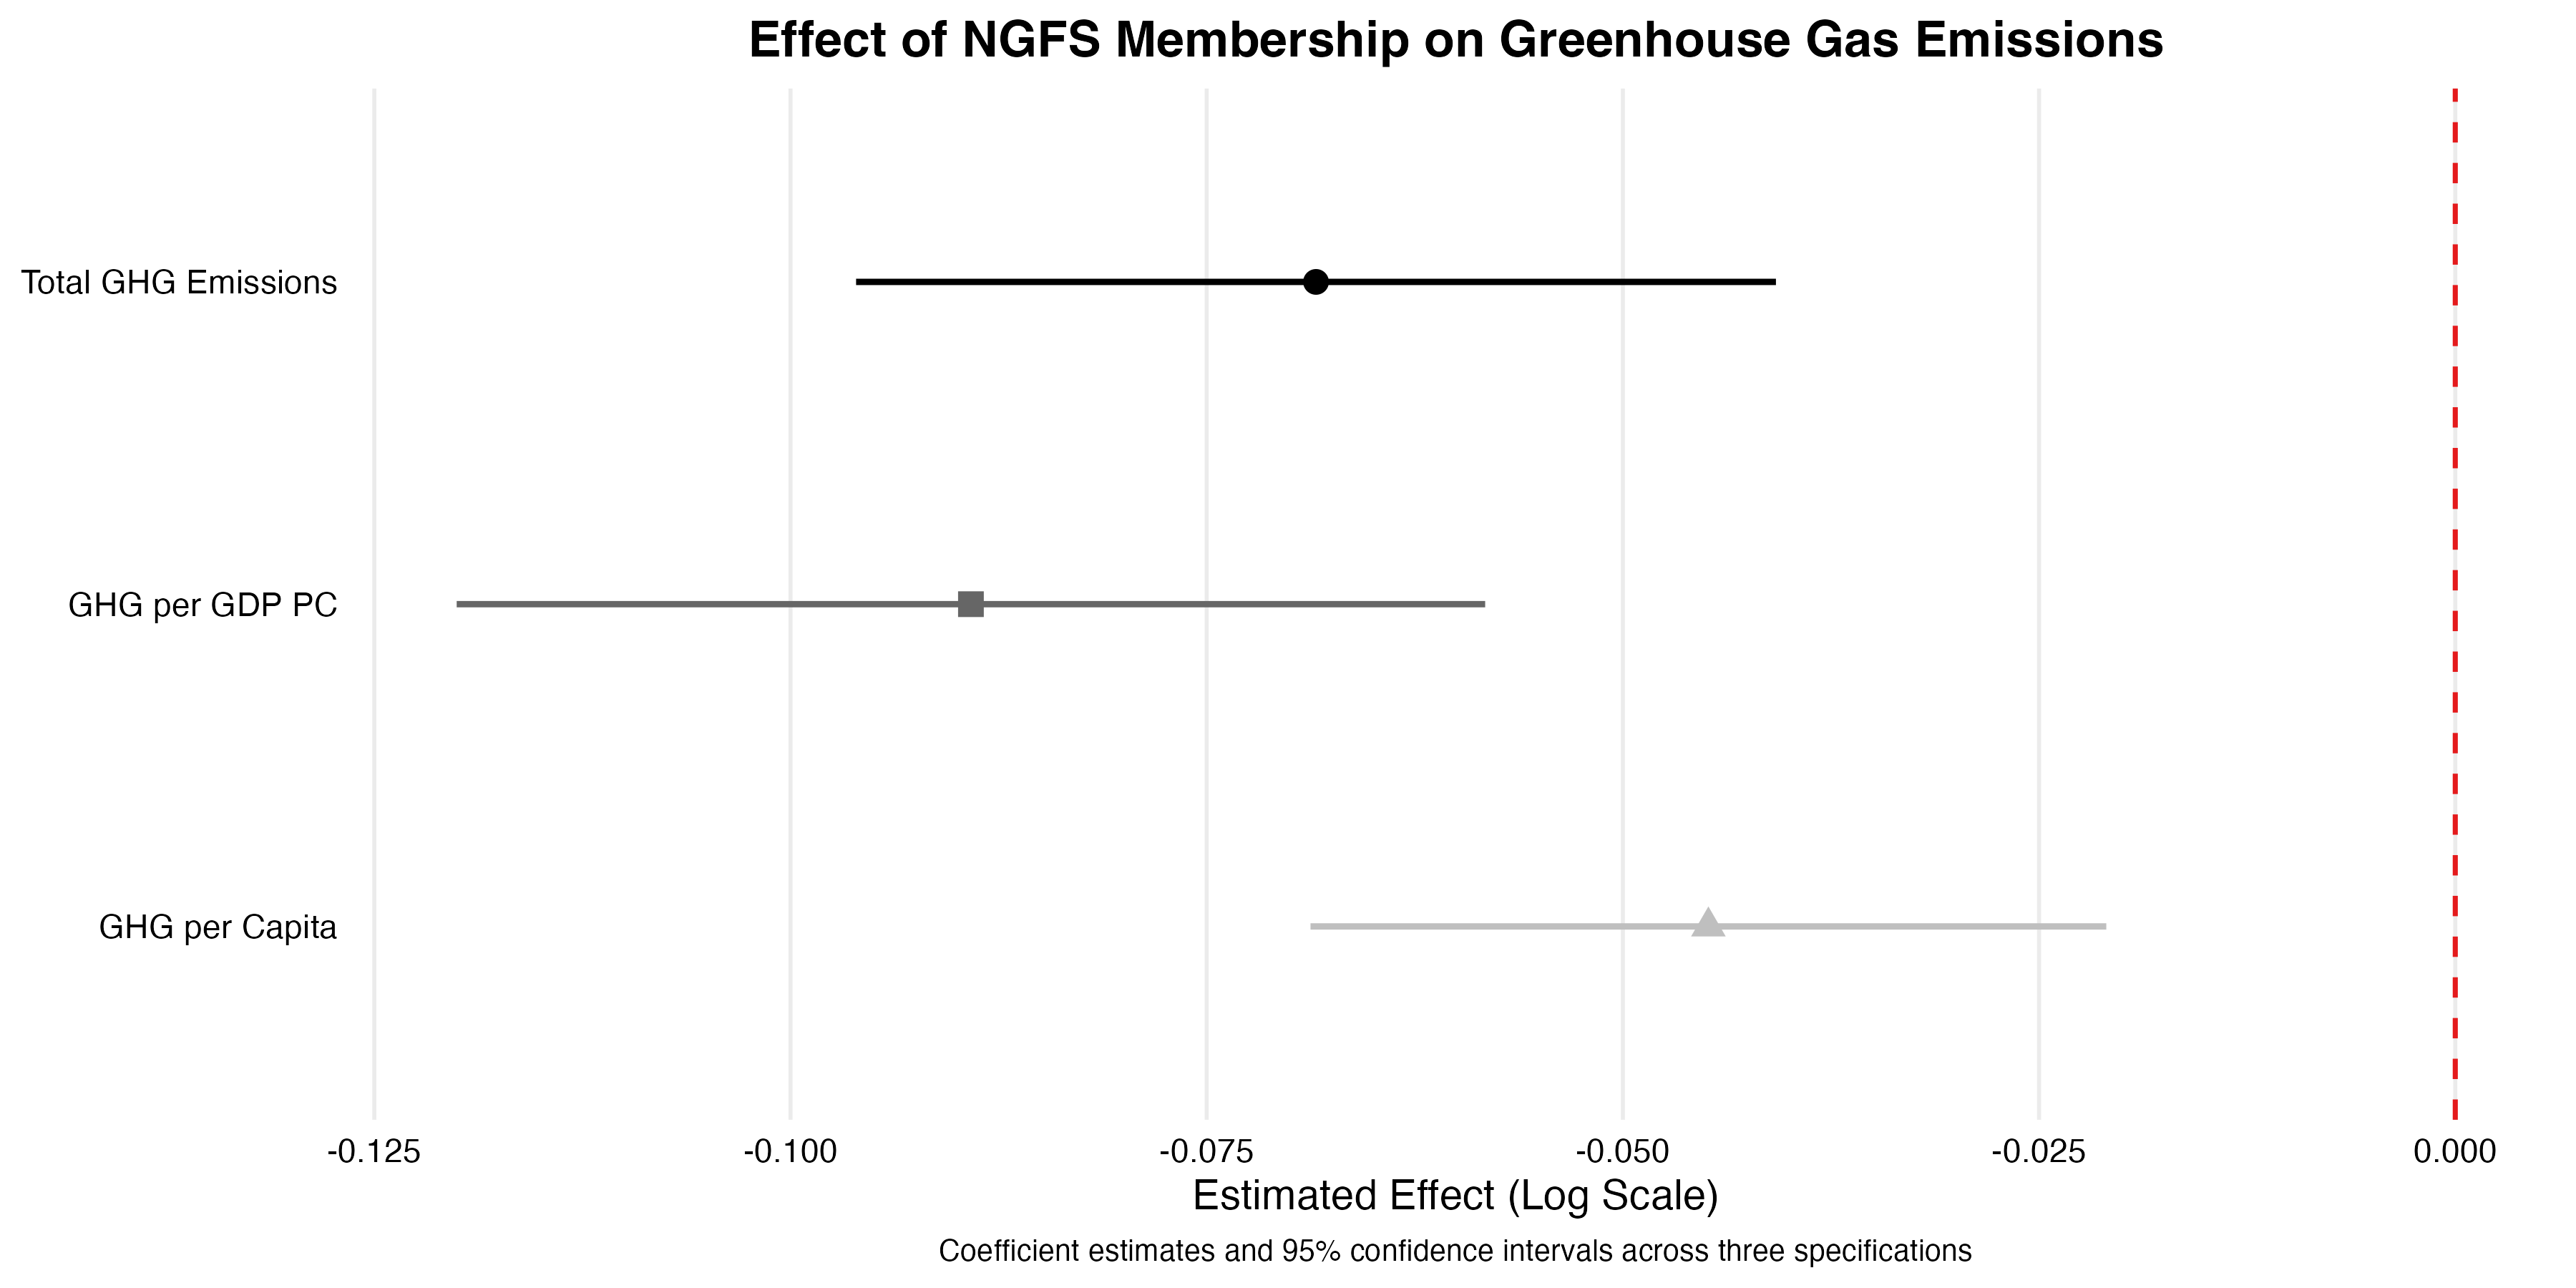
\includegraphics[keepaspectratio]{feplot.png}}

}

\caption{\label{fig-feplot}}

\end{figure}%

\textbf{\emph{Standard TWFE estimates can be vulnerable to bias under
staggered adoption; a doubly robust event-study design addresses both
timing heterogeneity and selection concerns}}

Yet, two main challenges complicate the TWFE results displayed in
Fig.~\ref{fig-feplot}. First, countries joined the NGFS at different
times---i.e., observations had a staggered adoption of the NGFS
treatment. France co-founded the network in 2017, Indonesia joined in
2019, Jordan in 2021, and so on. Also, recent work shows that TWFE can
produce biased estimates when treatment effects are heterogeneous across
adoption cohorts (\emph{12}, \emph{26}, \emph{27}). Second, early NGFS
members are disproportionately wealthy, industrialized economies,
raising the concern that any observed emissions gap reflects
pre-existing divergence rather than network membership.

To address both issues simultaneously, I employ Callaway and Sant'Anna's
doubly robust difference-in-differences estimator and aggregate the
resulting group-time average treatment effects using a dynamic
aggregation. This technique restricts comparisons to never-treated
countries and reweights observations via propensity scores to improve
pre-treatment comparability across cohorts. Fig.~\ref{fig-cs-event}
shows the CS dynamic estimates for various measures of emissions,
revealing a post-treatment downward trajectory across all three
specifications. The post-treatment decline is stronger and more
precisely estimated for total GHG emissions and GHG per GDP per capita
than for GHG per capita.

\begin{figure}[H]

\centering{

\pandocbounded{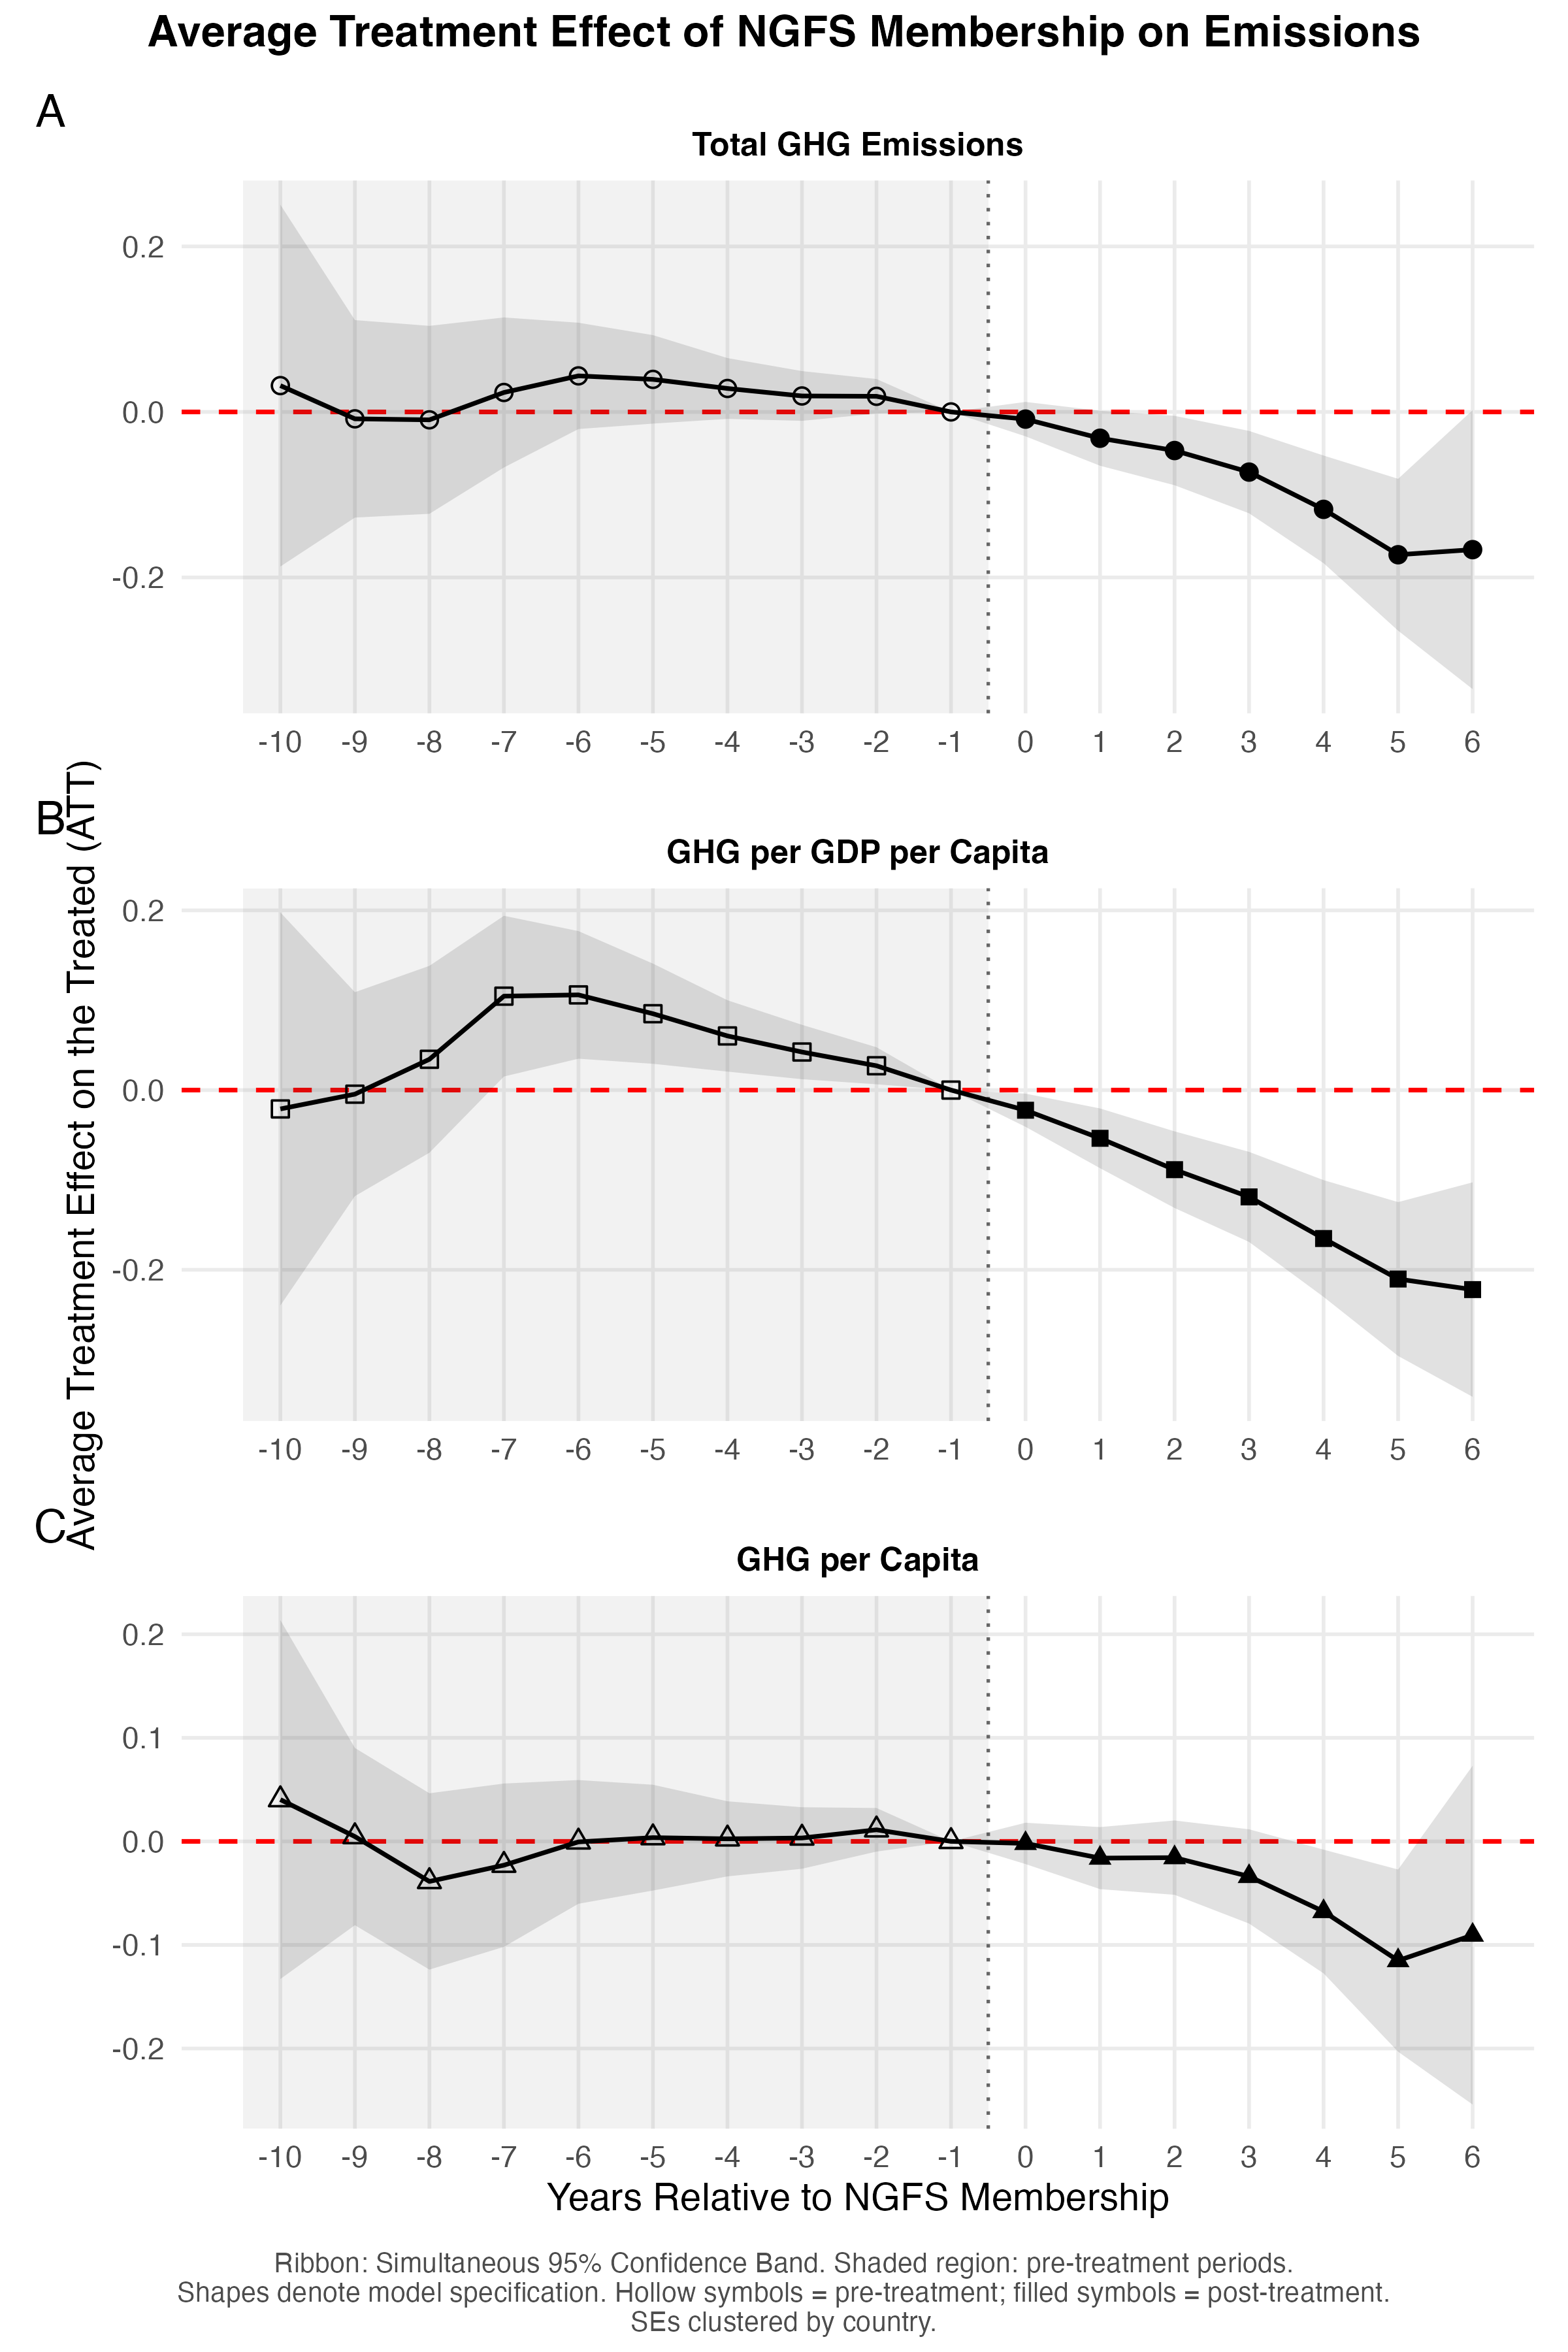
\includegraphics[keepaspectratio]{cs_plots_combined.png}}

}

\caption{\label{fig-cs-event}}

\end{figure}%

Pre-membership estimates, in turn, for emissions normalized per GDP per
capita reveal distinct trajectories. The observable differences
potentially stem from early-joiners being wealthier, more industrialized
nations than late-joiners and never-treated countries (see
Fig.~\ref{fig-comb-plot}). This point warrants an honest
acknowledgement: Pre-tests of parallel trends reveal statistically
significant effects particularly among early-joiners between 2013 and
2015, violating the parallel trends assumptions (\(p \approx 0\)). I
further conducted a formal sensitivity analysis (\emph{26}), which shows
that the overall effect on GHG emissions is robust to modest violations
of parallel trends (\(\bar{M} \approx 0.13\)). However, the effect does
not resist violations comparable in size to the largest pre-treatment
deviation (see Supplementary Materials).

At the same time, Fig.~\ref{fig-comb-plot} details how the pre-treatment
estimates follow a slight positive-to-zero decline in the two to three
years before treatment. The estimates within three years of treatment
are small and statistically indistinguishable from zero across all
cohorts. This feature, combined with the results of the senstivity
analysis, provides relevant parallel trends evidence while considering
the overall violation of the parallel trends concentrated in the early
cohorts.

In sum, the findings are consistent with a modest pre-existing
convergence between NGFS members and the never-treated control group.
Also, the average treatment effect on the treated (ATT) group is
significant and in the same direction as the TWFE results displayed in
Fig.~\ref{fig-feplot}. The ATT for emissions reduction are found in the
magnitude of 8\% for overall emissions (\(p < 0.05\)), 13\% for
emissions per GDP per capita (\(p < 0.1\)), and 5\% for emissions per
capita (\(p < 0.05\)). Additionally, the observed data on cohort
trajectories shown in Fig.~\ref{fig-comb-plot} confirm that neither
early-joiners nor late-joiners display a pronounced pre-existing
downward trend in median emissions. Indeed, the doubly robust
reweighting is designed to address the selection on observable
pre-treatment characteristics. Therefore, the post-treatment effect
identified in Fig.~\ref{fig-cs-event} should be interpreted as an
accelerated deceleration in emission growth relative to trend, not a
clean structural break from a perfectly flat baseline.

\textbf{\emph{Central bank independence conditions the magnitude of the
NGFS effect}}

The TWFE and DID results indicate that, all else equal, NGFS membership
is associated with average lower within-country emissions. I argue that
the capacity of central banks to translate international climate
commitments into domestic regulatory action depends on their insulation
from political interference (\emph{5}, \emph{7}, \emph{10}, \emph{16},
\emph{21}). To test this argument, I interact NGFS membership with a
Garriga's (\emph{14}) weighted central bank independence (CBI) index and
estimate marginal effects across the observed range of CBI scores.

Fig.~\ref{fig-cbi-margins} reveals that the marginal effect of NGFS
membership is a downward-sloping gradient across the CBI distribution,
not a threshold or a discontinuity. At low central bank independence
levels (one standard deviation below the global mean,
\(CBI \approx 0.42\)), NGFS membership is associated with a 3.3\%
reduction in emissions (\(\beta = -0.03\), \(SE = 0.02\), \(p < 0.05\)).
At the global mean (\(CBI \approx 0.62\)), the reduction increases to
approximately 6.0\% (\(\beta = -0.06\), \(SE = 0.01\), \(p < 0.001\)).
Among countries with highly independent central banks
(\(CBI \approx 0.81\)), the estimated NGFS membership effect reaches
about 8.7\% (\(\beta = -0.09\), \(SE = 0.02\), \(p < 0.001\)). As the
confidence band crosses zero at the lower tail of the CBI distribution,
this indicates that membership carries little statistically reliable
impact where central banks are most constrained by executive power.
Fig.~\ref{fig-cbi-pred} illustrates a similar pattern in predicted
emission levels: the gap between NGFS members and non-members widens
progressively as CBI rises, with statistically reliable divergence
beginning at \(CBI \approx 0.41\).

\begin{figure}[H]

\centering{

\pandocbounded{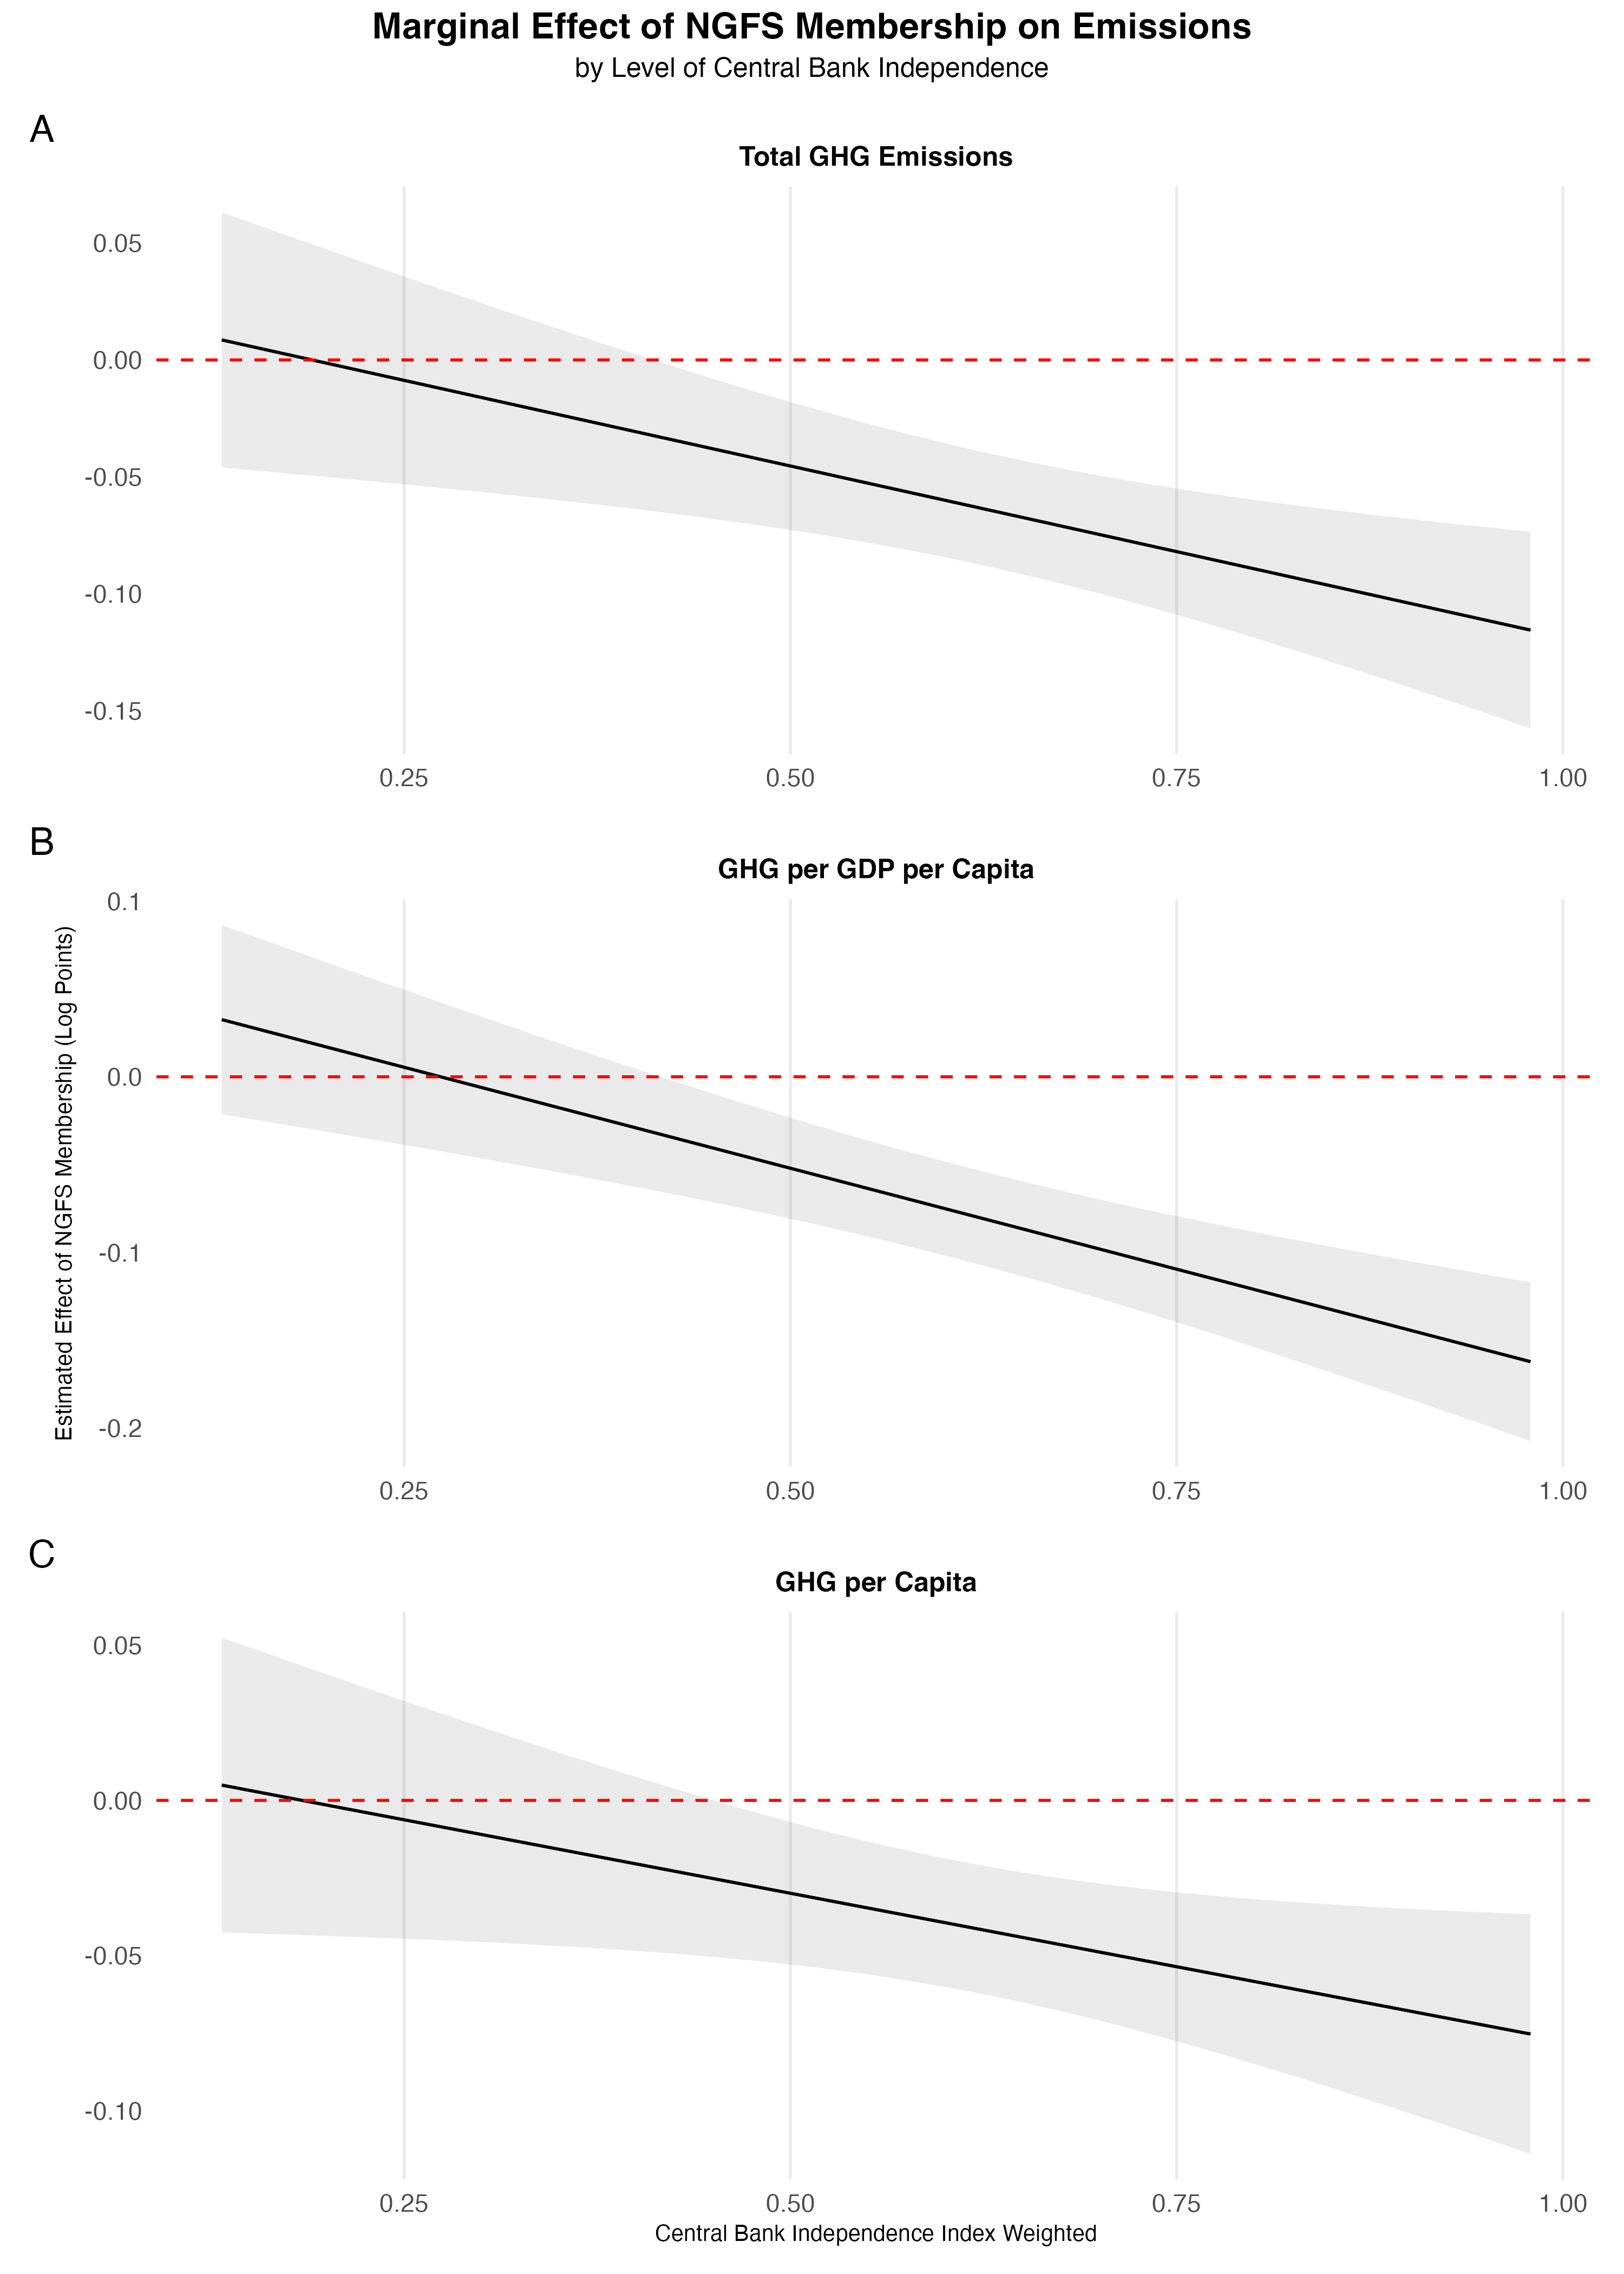
\includegraphics[keepaspectratio]{cbi_margins_plot.png}}

}

\caption{\label{fig-cbi-margins}}

\end{figure}%

\begin{figure}[H]

\centering{

\pandocbounded{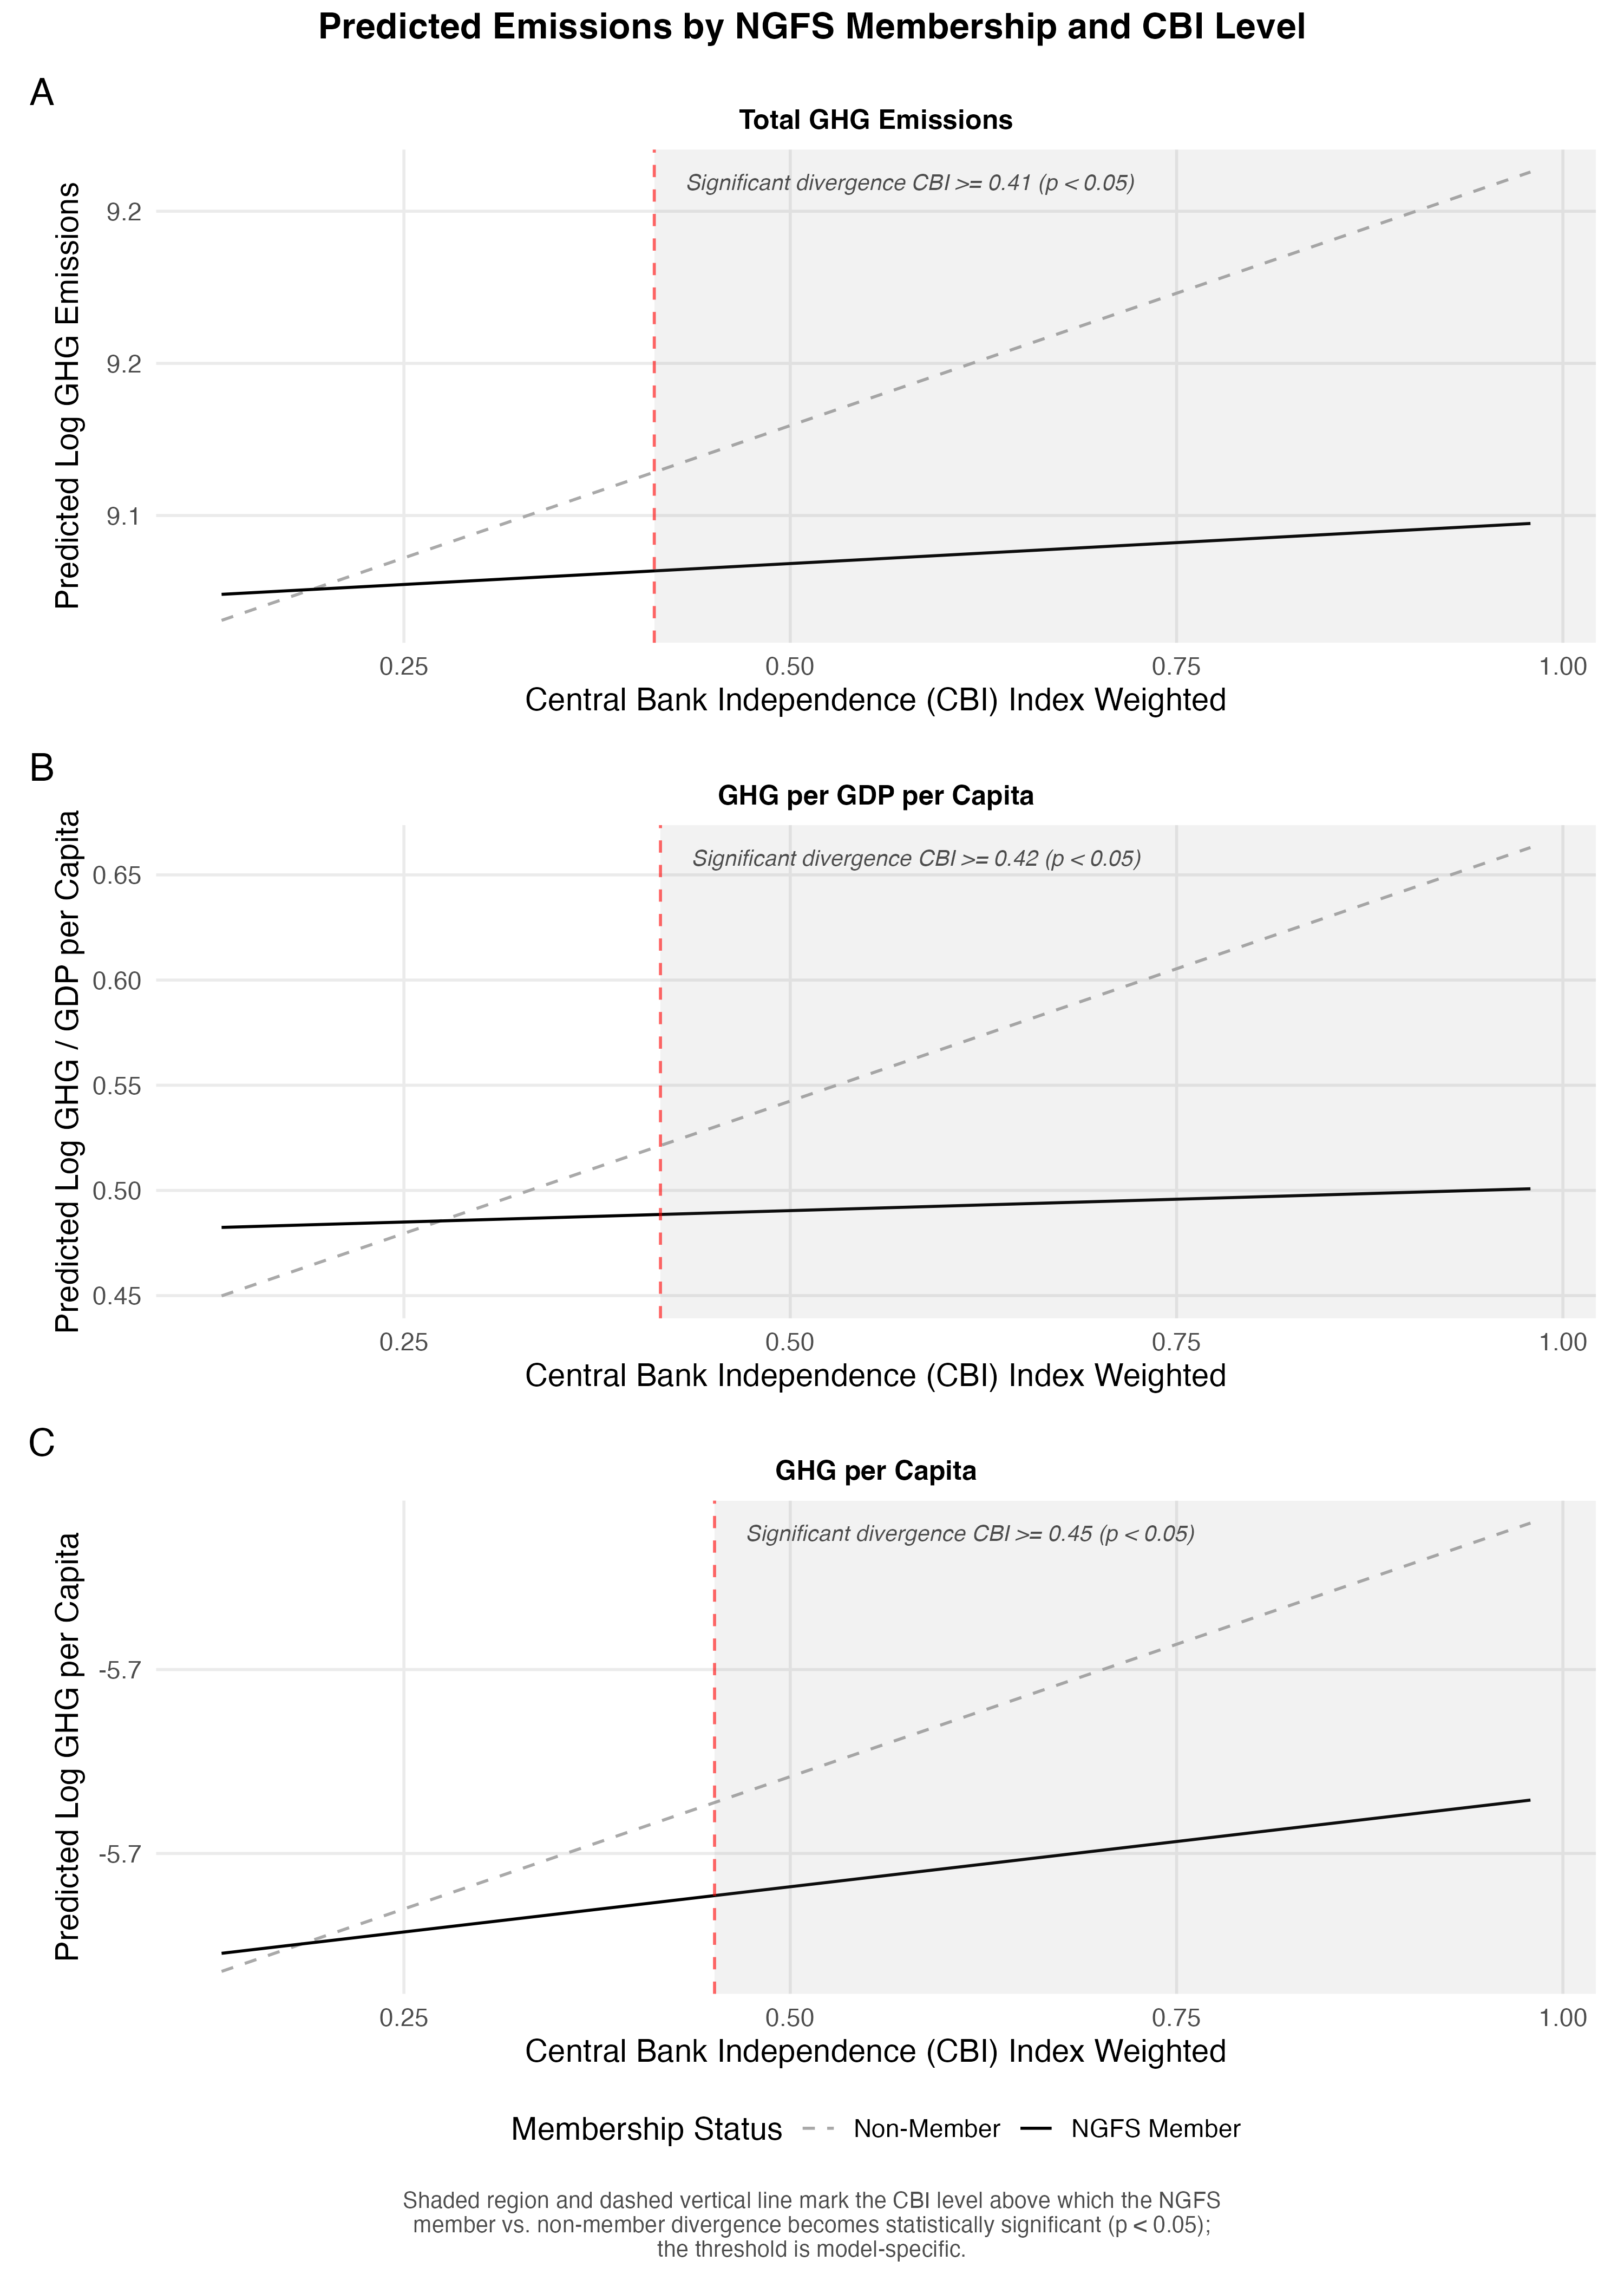
\includegraphics[keepaspectratio]{cbi_predictions_plot.png}}

}

\caption{\label{fig-cbi-pred}}

\end{figure}%

\textbf{\emph{Central bank independence functions as a moderating
condition, not as a mediating pathway activated by network membership}}

A plausible alternative mechanism is that joining the NGFS itself
strengthens a central bank's institutional autonomy. International
network membership may provide legitimacy, peer pressure, and technical
resources that insulate regulators from domestic political interference.
This autonomy, in turn, may enhance and then produce the emissions
reduction. To evaluate this mediation pathway, I conduct a causal
mediation analysis using two-way demeaned within-country variation, with
confidence intervals and p-values obtained from a cluster (block)
bootstrap that resamples whole countries rather than individual
country-years (see Supplementary Materials). The first-stage estimate
reveals that NGFS membership is associated with a small but
statistically significant \emph{decrease} in CBI (\(\beta = -0.01\),
\(p < 0.001\)), not an increase. This pattern potentially reflects the
coordination demands and institutional adjustments that network
participation in the NGFS requires. The indirect effect through CBI is
negligible in magnitude (proportion mediated \(\approx\) 0.2\%) and
statistically indistinguishable from zero (\(p = 0.82\)), with its point
estimate running counter to rather than reinforcing the overall
reduction. The dominant pathway is the average direct effect (ADE) of
NGFS membership (\(ADE = -0.03\), \(p < 0.001\)). Taken together, these
results indicate that pre-existing institutional autonomy amplifies the
NGFS effect, but network membership does not generate autonomy as a
byproduct. CBI is, therefore, a precondition for the network's
effectiveness in reducing within-country emissions, not a product of it.

Two features of this decomposition deserve a caveat. First, because CBI
and state capacity are themselves plausibly related institutional
features, each mediator model adjusts for the other candidate mediator:
the CBI models control for state capacity, and the state-capacity models
control for CBI. This choice isolates each pathway from the other, but
it assumes the two mediators do not share a causal relationship with one
another; if institutional capacity flows into central bank independence,
or vice versa, as part of the same underlying process, mutually
adjusting for both may partial out signal that a model treating them
jointly would retain. Second, as a check on this assumption, I repeat
the same decomposition using state capacity, rather than CBI, as the
candidate mediator. NGFS membership is not significantly associated with
within-country state capacity (\(\beta = -0.01\), \(p = 0.20\)), and the
resulting indirect effect is small and statistically indistinguishable
from zero (proportion mediated \(\approx\) 0.8\%, \(p = 0.58\)),
reinforcing the overall reduction just as the CBI pathway does. Neither
candidate mediator, in other words, is meaningfully shifted by NGFS
membership, which reinforces rather than merely accompanies the
conclusion reached through the CBI pathway above: pre-existing
institutional characteristics condition the network's effectiveness
rather than being manufactured by it.

\subsection{Discussion}\label{discussion}

This article asks whether countries with central banks formally
committed to climate-aligned financial regulation emit less greenhouse
gases than those without such commitment. Using NGFS membership as a
cross-nationally comparable treatment indicator, I find that, after
controlling for economic, ecological, and political factors,
within-country GHG emissions decelerate following network entry. The
reduction effect on emissions ranges from 4\% to 9\% depending on how
GHG is measured (fully-controlled specification, Fig.~\ref{fig-feplot}).
The effect is consistent across three emissions outcomes and is robust
to two identification checks that address serious identification
threats: heterogeneous treatment timing and endogenous selection into
the network. Three findings deserve special attention for what they
reveal about the mechanisms through which financial regulation, at the
global and national levels, contributes to decarbonization.

First, joining the NGFS in itself is significantly associated with
reduced emissions, but network membership alone is modest in absolute
terms. The observed data on cohort trajectories displayed in
Fig.~\ref{fig-comb-plot} show no substantial level shift in emissions
following network entry. Statistically, the effect on lowering emissions
is part of the within-country fixed-effects residual, reflecting a
deceleration of emission growth rather than an abrupt reduction. This is
consistent with how financial regulation operates. Central banks do not
function as environmental protection agencies or a ministry of the
environment. Financial supervisors do not mandate emission cuts
directly, but by gradually reshaping investment incentives, disclosure
requirements, and risk pricing in ways that compound over time. Still,
the modest magnitude of the effect in a seven-year window analyzed here
should not be mistaken for evidence that financial regulation is
unimportant; it may instead reflect the early stage of NGFS
institutionalization during the study period, which might keep producing
positive externalities for late joiners to continue reducing their
emissions moving forward.

Second, the moderation by central bank independence has direct policy
implications. The results shown in Fig.~\ref{fig-cbi-margins} indicate
that NGFS membership does not affect all nations uniformly. The positive
ramifications stemming from NGFS membership are largely concentrated
among countries whose central banks can translate international climate
commitments into binding domestic regulatory action as freely from
political interference as possible. This finding speaks to a broader
literature on the conditions under which international institutional
membership produces domestic policy change (CITE). The NGFS is a
voluntary, non-binding network. Its influence operates through
deliberations, agenda-setting, and other incentives rather than legal
obligations produced by hard international law. Where central banks lack
the autonomy to act independently from executive power, membership may
remain closer to a ``performative governance'' scenario (\emph{24}).

Third, the mediation results complicate a narrative that joining the
NGFS itself builds institutional capacity to reduce emissions by
connecting central banks to international peers and resources (\emph{1},
\emph{4}, \emph{10}). Instead, the evidence here suggests that NGFS
membership is associated with a slight \emph{reduction} in measured CBI.
This finding is consistent with the view that network participation
requires coordination and deference to shared standards that may
modestly constrain domestic, unilateral regulatory discretion. At the
same time, the dominant pathway from NGFS membership to emissions is
direct, i.e., through the regulatory and supervisory channels the
network establishes, rather than through a feedback loop that first
builds domestic autonomy.

These conclusions have noteworthy limitations. The statistical analysis
ends in 2021, capturing at most four post-treatment years for the
founding members and fewer for later joiners. The event-study estimates
show that the emissions reduction continues to deepen through year
three. This trend suggests that the full long-run effect may be larger
than what is estimable here. Extending the analysis period could yield
more comprehensive insights and check whether the effect persists beyond
the examined timeframe. My assessment also treats NGFS membership as a
binary indicator, obscuring variation in the depth of implementation
across members. For instance, Brazil devised a binding PRSAC mandate
(\emph{16}), whereas the U.S. Federal Reserve's presented a more
constrained engagement. Such contrast represents very different degrees
of practical commitment that a single membership dummy variable cannot
capture. Future research drawing from qualitative insights, case
studies, and implementation-quality data could better identify causal
mechanisms within the NGFS's broad treatment indicator used here.

Even considering these caveats, the results have a clear implication:
financial regulation is a meaningful instrument of climate policy, but
its effectiveness is conditioned on the international and domestic
institutional frameworks within which financial regulators operate.
Efforts to expand the NGFS and similar networks may produce greater
emissions reductions where they are paired with, or preceded by,
investments in central bank institutional capacity and bureaucratic
autonomy. For countries in the Global South, where both NGFS membership
is still growing and central bank independence remains lower on average,
the remaining questions about which conditions may further enable
emissions reduction is not merely academic. It has practical
consequences for how international climate finance governance should be
designed for the global economy to move toward decarbonization as
countries in the Global North and Global South alike pursue their
net-zero goals.

\{\{pagebreak\}\}

\subsection{References}\label{references}

\singlespacing

\protect\phantomsection\label{refs}
\begin{CSLReferences}{0}{1}
\bibitem[\citeproctext]{ref-battiston2021}
\CSLLeftMargin{1. }%
\CSLRightInline{S. Battiston, I. Monasterolo, K. Riahi, B. J. van
Ruijven, \href{https://doi.org/10.1126/science.abf3877}{Accounting for
{Finance Is Key} for {Climate Mitigation Pathways}}. \emph{Science}
\textbf{372}, 918--920 (2021).}

\bibitem[\citeproctext]{ref-boneva2022}
\CSLLeftMargin{2. }%
\CSLRightInline{L. Boneva, G. Ferrucci, F. P. Mongelli,
\href{https://doi.org/10.1080/14693062.2022.2070119}{Climate {Change}
and {Central Banks}: {What Role} for {Monetary Policy}?} \emph{Climate
Policy} \textbf{22}, 770--787 (2022).}

\bibitem[\citeproctext]{ref-dombret2021}
\CSLLeftMargin{3. }%
\CSLRightInline{A. Dombret, P. S. Kenadjian, \emph{Green {Banking} and
{Green Central Banking}} (Walter de Gruyter GmbH \& Co KG, 2021;
\url{https://books.google.com?id=48xMEAAAQBAJ}).}

\bibitem[\citeproctext]{ref-keenan2019}
\CSLLeftMargin{4. }%
\CSLRightInline{J. M. Keenan,
\href{https://doi.org/10.1126/science.aay8442}{A {Climate Intelligence
Arms Race} in {Financial Markets}}. \emph{Science} \textbf{365},
1240--1243 (2019).}

\bibitem[\citeproctext]{ref-amsden2001}
\CSLLeftMargin{5. }%
\CSLRightInline{A. H. Amsden, \emph{The {Rise} of "{The Rest}":
{Challenges} to the {West} from {Late-Industrializing Economies}}
(Oxford University Press, 2001).}

\bibitem[\citeproctext]{ref-sabel2024}
\CSLLeftMargin{6. }%
\CSLRightInline{C. F. Sabel, D. G. Victor, \emph{Fixing the {Climate}:
{Strategies} for an {Uncertain World}} (Princeton University Press,
Princeton, 2024).}

\bibitem[\citeproctext]{ref-wade1990}
\CSLLeftMargin{7. }%
\CSLRightInline{R. Wade, \emph{Governing the {Market}: {Economic Theory}
and the {Role} of {Government} in {East Asian Industrialization}}
(Princeton University Press, 1990).}

\bibitem[\citeproctext]{ref-zysman1983}
\CSLLeftMargin{8. }%
\CSLRightInline{J. Zysman, \emph{Governments, {Markets}, and {Growth}:
{Financial Systems} and the {Politics} of {Industrial Change}} (Cornell
University Press, 1983).}

\bibitem[\citeproctext]{ref-campiglio2018}
\CSLLeftMargin{9. }%
\CSLRightInline{E. Campiglio, Y. Dafermos, P. Monnin, J. Ryan-Collins,
G. Schotten, M. Tanaka,
\href{https://doi.org/10.1038/s41558-018-0175-0}{Climate {Change
Challenges} for {Central Banks} and {Financial Regulators}}.
\emph{Nature Clim Change} \textbf{8}, 462--468 (2018).}

\bibitem[\citeproctext]{ref-helleiner2025}
\CSLLeftMargin{10. }%
\CSLRightInline{E. Helleiner, M. DiLeo, J. van 't Klooster,
\href{https://doi.org/10.1111/rego.12629}{Financial {Technocrats} as
{Competitive Regime Creators}: {The Founding} and {Design} of the
{Network} for {Greening} the {Financial System}}. \emph{Regulation \&
Governance} \textbf{Online First} (2025).}

\bibitem[\citeproctext]{ref-ngfs2025}
\CSLLeftMargin{11. }%
\CSLRightInline{NGFS, Origin and {Purpose} (2025).
\url{https://www.ngfs.net/en/about-us/origin-and-purpose}.}

\bibitem[\citeproctext]{ref-callaway2021}
\CSLLeftMargin{12. }%
\CSLRightInline{B. Callaway, P. H. C. Sant'Anna,
\href{https://doi.org/10.1016/j.jeconom.2020.12.001}{Difference-in-{Differences}
with {Multiple Time Periods}}. \emph{Journal of Econometrics}
\textbf{225}, 200--230 (2021).}

\bibitem[\citeproctext]{ref-garriga2016}
\CSLLeftMargin{13. }%
\CSLRightInline{A. C. Garriga,
\href{https://doi.org/10.1080/03050629.2016.1188813}{Central {Bank
Independence} in the {World}: {A New Data Set}}. \emph{International
Interactions} \textbf{42}, 849--868 (2016).}

\bibitem[\citeproctext]{ref-garriga2025}
\CSLLeftMargin{14. }%
\CSLRightInline{A. C. Garriga,
\href{https://doi.org/10.1093/isq/sqaf024}{Revisiting {Central Bank
Independence} in the {World}: {An Extended Dataset}}. \emph{Int Stud Q}
\textbf{69}, sqaf024 (2025).}

\bibitem[\citeproctext]{ref-bersch2023}
\CSLLeftMargin{15. }%
\CSLRightInline{K. Bersch, F. Fukuyama, Defining {Bureaucratic
Autonomy}. \emph{Annual Review of Political Science} \textbf{26}, 213
(2023).}

\bibitem[\citeproctext]{ref-dias2026}
\CSLLeftMargin{16. }%
\CSLRightInline{V. M. Dias, M. G. Schapiro,
\href{https://doi.org/10.1111/psj.70101}{Resisting {Democratic
Backsliding From Within} the {State}: {Environmental Politics} in
{Bolsonaro}'s {Brazil}}. \emph{Policy Studies Journal} \textbf{n/a}
(2026).}

\bibitem[\citeproctext]{ref-mcdonnell2020}
\CSLLeftMargin{17. }%
\CSLRightInline{E. M. McDonnell, \emph{Patchwork {Leviathan}: {Pockets}
of {Bureaucratic Effectiveness} in {Developing States}} (Princeton
University Press, Princeton, 2020).}

\bibitem[\citeproctext]{ref-dincer2024}
\CSLLeftMargin{18. }%
\CSLRightInline{N. Dincer, B. Eichengreen, J. J. Martinez,
\href{https://doi.org/10.1146/annurev-economics-081623-032553}{Central
{Bank Independence}: {Views} from {History} and {Machine Learning}}.
\emph{Annual Review of Economics} \textbf{16}, 393--428 (2024).}

\bibitem[\citeproctext]{ref-fernandez-albertos2015}
\CSLLeftMargin{19. }%
\CSLRightInline{J. Fernández-Albertos,
\href{https://doi.org/10.1146/annurev-polisci-071112-221121}{The
{Politics} of {Central Bank Independence}}. \emph{Annual Review of
Political Science} \textbf{18}, 217--237 (2015).}

\bibitem[\citeproctext]{ref-hayo2008}
\CSLLeftMargin{20. }%
\CSLRightInline{B. Hayo, S. Voigt, Inflation, {Central Bank
Independence}, and the {Legal System}. \emph{Journal of Institutional
and Theoretical Economics (JITE) / Zeitschrift für die gesamte
Staatswissenschaft} \textbf{164}, 751--777 (2008).}

\bibitem[\citeproctext]{ref-evans1995}
\CSLLeftMargin{21. }%
\CSLRightInline{P. B. Evans, \emph{Embedded {Autonomy}: {States} and
{Industrial Transformation}} (Princeton University Press, Princeton,
N.J., 1995).}

\bibitem[\citeproctext]{ref-wef2026}
\CSLLeftMargin{22. }%
\CSLRightInline{World Economic Forum, The {Global Risks Report} 2026
(2026).
\url{https://www.weforum.org/publications/global-risks-report-2026/digest/}.}

\bibitem[\citeproctext]{ref-meckling2011}
\CSLLeftMargin{23. }%
\CSLRightInline{J. Meckling, \emph{Carbon {Coalitions}: {Business},
{Climate Politics}, and the {Rise} of {Emissions Trading}} (MIT Press,
2011; \url{https://books.google.com?id=dtyO6mcrh5EC}).}

\bibitem[\citeproctext]{ref-ding2020}
\CSLLeftMargin{24. }%
\CSLRightInline{I. Ding,
\href{https://doi.org/10.1017/S0043887120000131}{Performative
{Governance}}. \emph{World Politics} \textbf{72}, 525--556 (2020).}

\bibitem[\citeproctext]{ref-hafner-burton2005}
\CSLLeftMargin{25. }%
\CSLRightInline{E. M. Hafner-Burton, K. Tsutsui, Human {Rights} in a
{Globalizing World}: {The Paradox} of {Empty Promises}. \emph{American
Journal of Sociology} \textbf{110}, 1373--1411 (2005).}

\bibitem[\citeproctext]{ref-rambachan2023}
\CSLLeftMargin{26. }%
\CSLRightInline{A. Rambachan, J. Roth,
\href{https://doi.org/10.1093/restud/rdad018}{A {More Credible Approach}
to {Parallel Trends}}. \emph{Rev Econ Stud} \textbf{90}, 2555--2591
(2023).}

\bibitem[\citeproctext]{ref-sun2021}
\CSLLeftMargin{27. }%
\CSLRightInline{L. Sun, S. Abraham,
\href{https://doi.org/10.1016/j.jeconom.2020.09.006}{Estimating {Dynamic
Treatment Effects} in {Event Studies} with {Heterogeneous Treatment
Effects}}. \emph{Journal of Econometrics} \textbf{225}, 175--199
(2021).}

\end{CSLReferences}




\end{document}
